\documentclass[12pt, a4paper]{report}
\usepackage{graphicx}
\usepackage{amsmath}
\usepackage{float}
\renewcommand{\baselinestretch}{1.2} 
\usepackage{ragged2e}
\usepackage{fancyvrb}
\usepackage{amssymb}
\usepackage[a4paper, total={7in, 9in}]{geometry}
\usepackage[utf8]{inputenc}
\usepackage{physics}
\usepackage{enumitem}


\title{\textbf{EE2703 : Applied Programming Lab \\ Assignment 5 \\ The Resistor Problem}} % Title
\author{Arun Krishna A M S \\ EE19B001} % Author name

\date{\today} % Date for the report

\begin{document}		
		
\maketitle % Insert the title, author and date
\justifying

\section*{Aim}
A resistor is a passive two-terminal electrical component that implements electrical resistance as a circuit element. Resistors are common elements of electrical networks and electronic circuits and are ubiquitous in electronic equipment. Practical resistors as discrete components can be composed of various compounds and forms. In this assignment, we mainly focus on:
\begin{itemize}
  	\item Finding the potential on each point on the resistor through Laplace's equation by numerical methods
  	\item Determining the profile of the current flowing through the resistor i.e.,dependence of current on the shape of the resistor
  	\item Find which part of the resistor is likely to get hottest, by solving Poisson's equation numerically
  	\item Vectorization of for-loops for faster computing
\end{itemize}

\section*{Introduction}
Consider the following apparatus:
A wire is soldered to the middle of a copper plate and its voltage is held at 1 Volt. One side of the plate is grounded, while the remaining are floating. The plate is 1 cm by 1 cm in size.
\begin{center}
	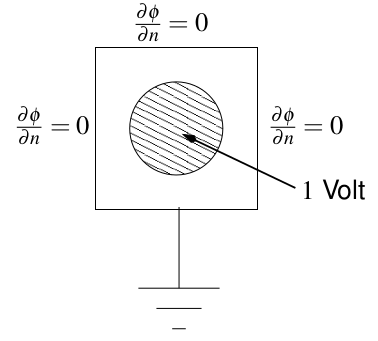
\includegraphics[scale=0.60]{Figure1} 
	\caption{\\Apparatus}
	\label{fig:rawdata}
\end{center}

As a result of the potential difference, current flows - given by the current density $\overrightarrow{J}$. This current density is related to the local electric field by Ohm’s Law:
\begin{equation*}
\overrightarrow{J} = \sigma \overrightarrow{E}
\end{equation*}
The \textbf{continuity equation} states:
\begin{equation*}
\nabla.\overrightarrow{J} = -\frac{\partial\rho}{\partial t}
\end{equation*}
and we know that, the electric field varies with electrostatic potential as
\begin{equation*}
\overrightarrow{E} = -\nabla\phi
\end{equation*}
Combining the above three equations we arrive at
\begin{equation*}
\nabla.(-\sigma\nabla\phi) = -\frac{\partial\rho}{\partial t}
\implies \nabla^2\phi = \frac{1}{\sigma}\frac{\partial\rho}{\partial t} 
\end{equation*}
Where $\sigma$ is the material's constant conductivity. For DC currents, the right hand side is zero, and we obtain the \textbf{laplace equation}:
\begin{equation*}
\nabla^2\phi = 0
\end{equation*}
This equation is a special case of Poisson's equation: 
\begin{equation*}
\nabla^2\phi = f
\end{equation*}
Laplace's equation in two-dimensions can  be written in Cartesian coordinates as 
\begin{equation*}
\frac{\partial^2 \phi}{\partial x^2} + \frac{\partial^2 \phi}{\partial y^2} = 0
\end{equation*}
When written in discrete form
 \begin{align*}
 \frac{\partial \phi}{\partial x}\Bigr|_{\substack{(x_i,y_j)}} = \frac{\phi(x_{i+1/2},y_j) - \phi(x_{i-1/2},y_j)}{\triangle x} \\
 \frac{\partial^2 \phi}{\partial x^2}\Bigr|_{\substack{(x_i,y_j)}} = \frac{\phi(x_{i+1},y_j) -2\phi(x_i,y_j) +\phi(x_{i-1},y_j)}{\triangle x} 
 \end{align*}
 Similarly
\begin{align*}
\frac{\partial^2 \phi}{\partial y^2}\Bigr|_{\substack{(x_i,y_j)}} = \frac{\phi(x_i,y_{j+1}) -2\phi(x_i,y_j) +\phi(x_i,y_{j-1})}{\triangle y}
 \end{align*}
Combining both equations, we arrive at
\begin{equation*}
\phi_{i,j} = \frac{\phi_{i,j-1}+\phi_{i-1,j}+\phi_{i+1,j}+\phi_{i,j+1}}{4} 
\end{equation*}
Thus, if the solution holds, the potential at any point should be the average of its neighbours. One can also argue that the function $\phi$ is a harmonic function, thus the result holds. 


\section*{Initialization}

We initialize the coordinate system as follows:
\begin{verbatim}
Nx = 50                 
Ny = 50
radius = 10
Niter = 1500
x = np.linspace(0.5,-0.5,Nx,dtype = float);
y = np.linspace(0.5,-0.5,Ny,dtype = float);
Y,X = np.meshgrid(y,x);
\end{verbatim}
\texttt{Nx} and \texttt{Ny} determine the resolution of the coordinate system, and \texttt{radius} determines the radius of the soldered wire. \texttt{X} and \texttt{Y} are used as a coordinate map for further code execution. 

The initial values of the system is determined by the conditions specified earlier. The area of contact of the wire to the middle of copper plate is at 1 Volt. We initialize electric potential \texttt{phi} as $0$ for all other points

\begin{verbatim}
radius = (1/Nx + 1/Ny)*(1/2)*radius;
ii = np.where(np.multiply(X,X) + np.multiply(Y,Y) < radius**2);
phi = np.zeros([Ny,Nx], dtype = float);
phi[ii] = 1.0;
\end{verbatim}

\begin{center}
	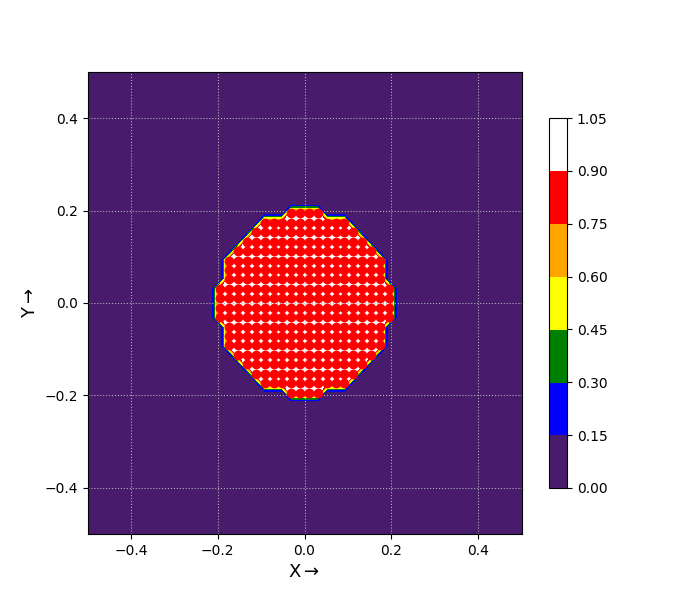
\includegraphics[scale=0.60]{Figure2} 
	\caption{\\Electric Potential - initial values}
	\label{fig:rawdata}
\end{center}

\section*{Boundary Condition and Laplace equation}

At boundaries where the electrode is present, the value of electrostatic potential is same as electrode potential itself. At the bottom boundary where the plate is connected to ground, the potential is always zero. At other boundaries the gradient of $\phi$ should be tangential i.e., $\phi$ should not vary in the normal direction. For example, at the left boundary, at $\frac{\partial \phi}{\partial n} = 0$. This is achieved by

\begin{verbatim}
phi[:, 0] = phi[:, 1];            #Left margin              
phi[:, Nx-1] = phi[:, Nx-2];      #Right margin
phi[0, :] = phi[1, :];            #Top margin
phi[Ny-1, :] = 0;                 #Bottom margin
phi[ii] = 1.0;                    #Potential = electrode potential = 1V
\end{verbatim}

As mentioned earlier, at each point, replace the potential by the average of its neighbours. Keep iterating till the solution converges.
\begin{verbatim}
oldphi = phi.copy()
phi[1:-1,1:-1] = 
0.25*(oldphi[1:-1,0:-2] + oldphi[1:-1,2:] + oldphi[0:-2,1:-1] + oldphi[2:,1:-1]);
\end{verbatim}

In each iteration, the $\phi$ value at each point is copied, and the potential is replaced by the average of its neighbours. The boundary condition is also enforced in each iteration. The error for each iteration is also calculated.
\begin{verbatim}
for k in range(Niter)
    save copy of phi
    update phi array
    assert boundaries
    errors[k]=(abs(phi-oldphi)).max();
#end
\end{verbatim}


\begin{center}
	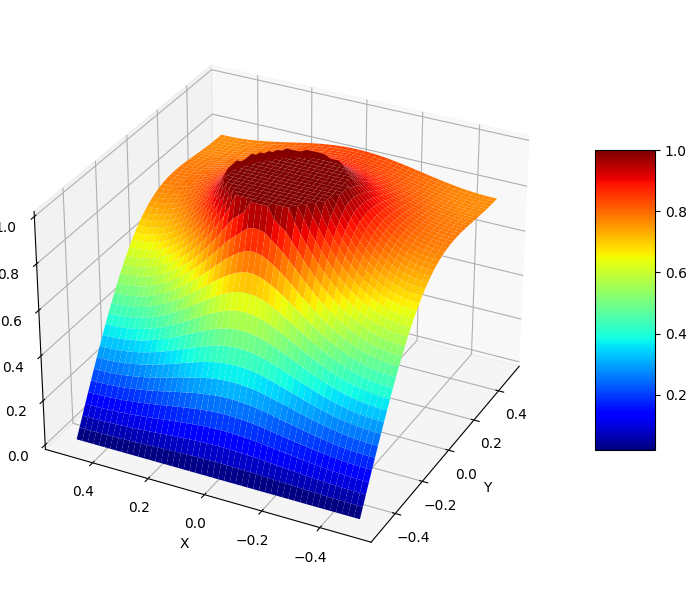
\includegraphics[scale=0.60]{Figure3} 
	\caption{\\3-D contour plot: Electrostatic Potential}
	\label{fig:rawdata}
\end{center}


\begin{center}
	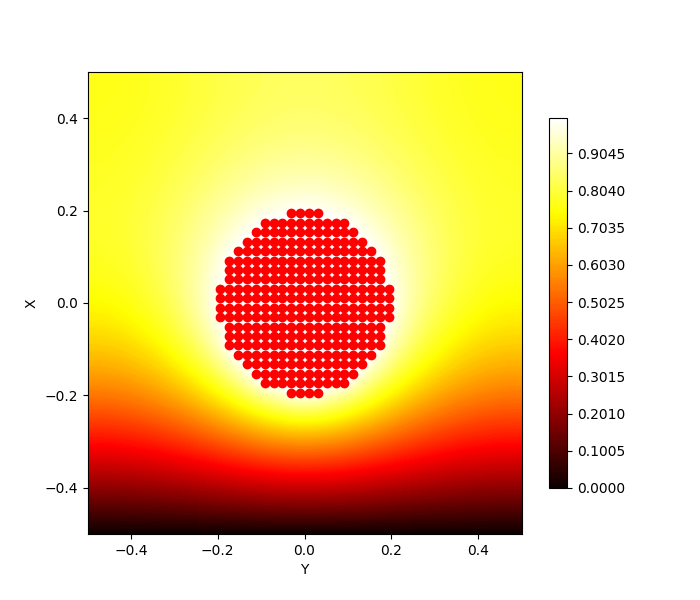
\includegraphics[scale=0.60]{Figure4} 
	\caption{\\2-D contour plot: Electrostatic Potential}
	\label{fig:rawdata}
\end{center}
The marked red dots is the area of contact between electrode and the copper plate.

\section*{Error Plot}
\begin{center}
	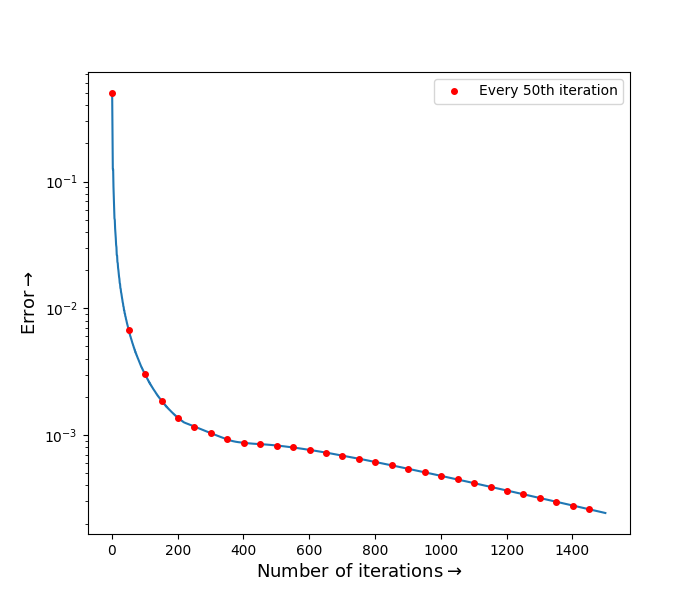
\includegraphics[scale=0.65]{Figure5} 
	\caption{\\Error vs Number of Iterations: semilogY plot}
	\label{fig:rawdata}
\end{center}
\begin{center}
	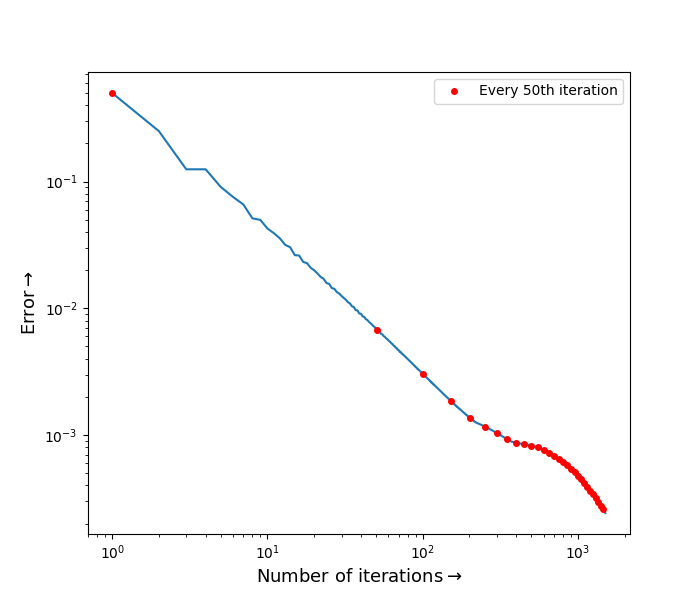
\includegraphics[scale=0.65]{Figure6} 
	\caption{\\Error vs Number of Iterations: loglog plot}
	\label{fig:rawdata}
\end{center}
We can find that a log-log plot gives a reasonably straight line upto about 500 iterations, but beyond that, it falls into the exponential regime. While plotting semilog plot, we can find that it is an exponential decay only for larger iteration numbers.

Since it is exponential, we extract the exponent and fit into a semilog plot of the form:
\begin{align*}
y = Ae^{bx} \\
\log y = \log A + b\log x
\end{align*}
 To estimate the values of $A$ and $b$ we use \textbf{least square method} such that the error in Y is minimum. 

\begin{equation*}
\begin{pmatrix}
1 & x_1\\
1 & x_2\\
1 & x_3\\
.  .\\
.  .\\
1 & x_n\\
\end{pmatrix}
.
\begin{pmatrix}
\log(A)\\
B\\
\end{pmatrix}
=
\begin{pmatrix}
\log(y_1)\\
\log(y_2)\\
.\\
.\\
\log(y_n)\\
\end{pmatrix}
\end{equation*}



Since, we find that it is an exponential decay only for larger iteration numbers, we try to fit the curve for both the entire vector and for iterations greater than 500.
\begin{verbatim}
def Fitting_Function(X,Y):
    logY = np.transpose(log(Y));
    X = np.c_[np.ones([np.size(X),1]),X];
    return scipy.linalg.lstsq(X,logY)[0];   

A1, B1 = Fitting_Function(iterations, errors);
A1 = exp(A1);
A2, B2 = Fitting_Function(iterations[500:], errors[500:]);
A2 = exp(A2);
print(A1, B1, A2, B2);
\end{verbatim}

The determined coefficients is then used to plot the error. From the graph we can see that the values of $A$ and $b$ estimated by considering iterations greater than 500 is accurate compared to fitting the curve using the entire vector.
\begin{center}
	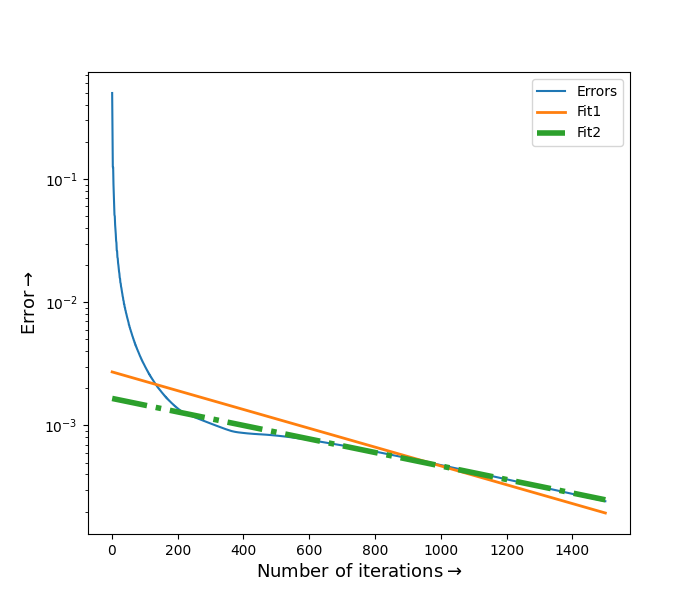
\includegraphics[scale=0.6]{Figure7} 
	\caption{\\Fitting errors: semilog plot}
	\label{fig:rawdata}
\end{center}
The cumulative error is given by:
\begin{equation*}
    \text{Cumulative error} = \sum_{k=N+1}^{\infty}Error < \int_{N+1}^{\infty}Ae^{bx} = \frac{A}{B}exp(B(N+0.5))
\end{equation*}
\begin{center}
	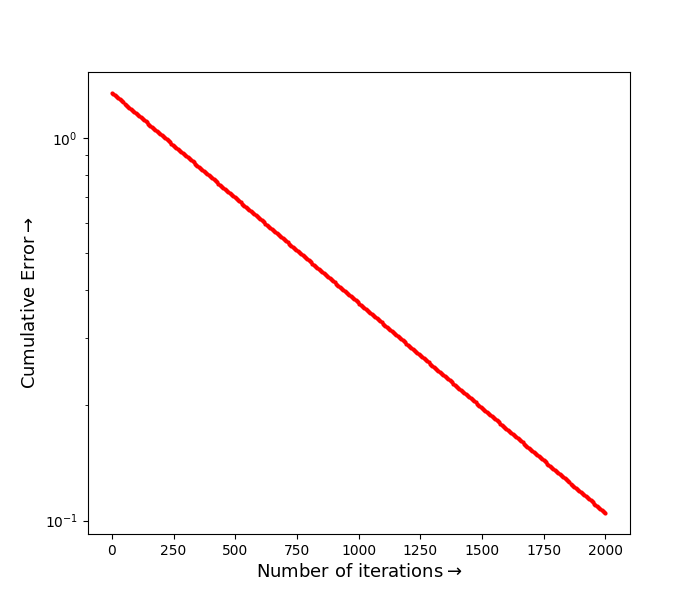
\includegraphics[scale=0.6]{Figure8} 
	\caption{\\Cumulative Error: semilogy plot}
	\label{fig:rawdata}
\end{center}
\begin{center}
	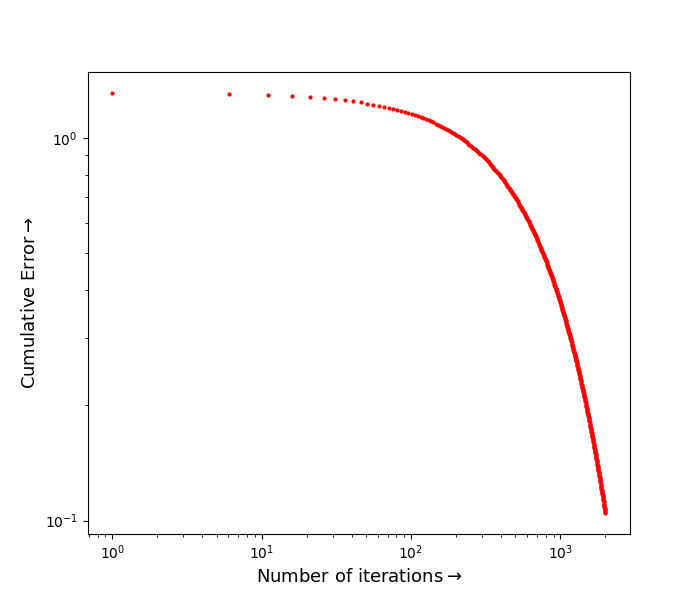
\includegraphics[scale=0.65]{Figure9} 
	\caption{\\Cumulative Error: loglog plot}
	\label{fig:rawdata}
\end{center}

\section*{Current Distribution}
To obtain the current profile, we compute the gradient. Since the major aim of this assignment is to find the shape of the current profile, we set the conductivity $\sigma$ to unity. The equations are then:

\begin{align*}
J_x = -\frac{\partial\phi}{\partial x} \\
J_y = -\frac{\partial\phi}{\partial y}
\end{align*}
This numerically translates to 
\begin{align*}
J_{x,ij} = \frac{1}{2}(\phi_{i,j-1} - \phi_{i,j+1}) \\
J_{y,ij} = \frac{1}{2}(\phi_{i,j-1} - \phi_{i,j+1})
\end{align*}

The arrays $J_x$ and $J_y$ are created. The current density is plotted using \texttt{quiver} function and the electrode is marked via red dots.
\begin{verbatim}
Jx = 1/2*(phi[1:-1,:-2]-phi[1:-1,2:])
Jy = 1/2*(phi[:-2,1:-1]-phi[2:,1:-1])
.
.
quiver(Y[1:-1,1:-1],X[1:-1,1:-1],-Jx,-Jy, label = "Current")
\end{verbatim}
\begin{center}
	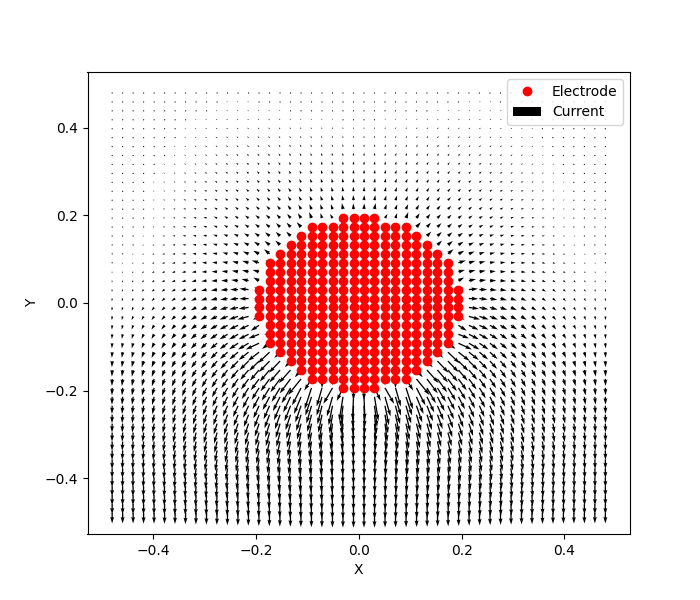
\includegraphics[scale=0.65]{Figure10} 
	\caption{\\Vector Plot: Current Distribution Profile}
	\label{fig:rawdata}
\end{center}
We can observe that the current flow is from higher potential(i.e., electrode 1V) to lower potential (ground). There is no current within the area of contact with electrode potential, since the electrostatic potential is constant i.e., 1V. Hardly any current flows to the top part of the copper plate.

\section*{Heat Map of the conductor}
Most of the current is in the bottom region, making the region relatively hot.
\begin{equation*}
\nabla.(\kappa\nabla T) = -\frac{1}{\sigma}|\overrightarrow{J}|^2
\end{equation*}
where the right side represents heat generated from ohmic loss. The above equation is a \textbf{Poisson's equation}. The boundary condition is $T=300$ at the wire and the ground while $\frac{\partial T}{\partial n} = 0$ at the other three edges.

\begin{verbatim}
temperature = 300*np.ones([Ny,Nx], dtype = float);
for k in range(Niter):
    oldtemperature = temperature.copy() 
    var = (Jx**2 + Jy**2);
    
    temperature[1:-1,1:-1]=0.25*(oldtemperature[1:-1,0:-2]+ oldtemperature[1:-1,2:]+
    oldtemperature[0:-2,1:-1] + oldtemperature[2:,1:-1] + var);
    
    temperature[:, 0] = temperature[:, 1];            #Left margin              
    temperature[:, Nx-1] = temperature[:, Nx-2];      #Right margin
    temperature[0, :] = temperature[1, :];            #Top margin
    temperature[Ny-1, :] = 300;                       #Bottom margin
    temperature[ii] = 300;                    
\end{verbatim}
\begin{center}
	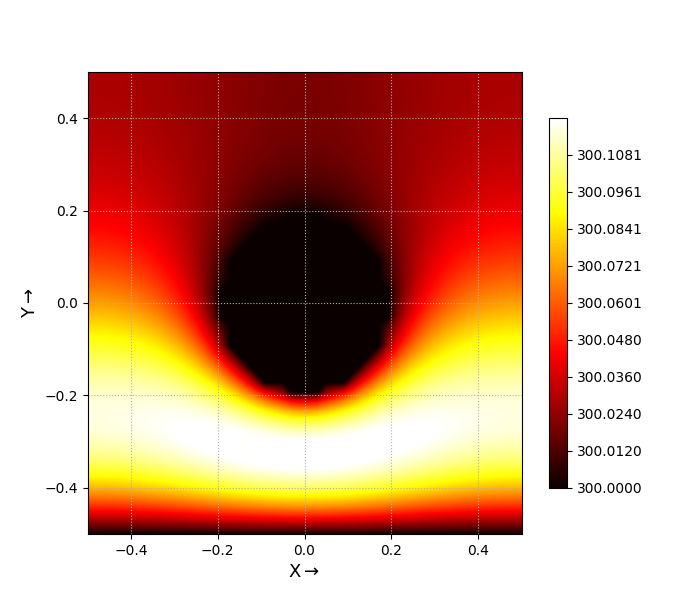
\includegraphics[scale=0.6]{Figure11} 
	\caption{\\Heat Signature: Temperature: Contour plot}
	\label{fig:rawdata}
\end{center}

\section*{Conclusion}
Solution for the Laplace's equation for the given system is found numerically. As the decay of error is very slow this method of solving Laplace’s equation is highly inefficient. Errors were plotted and we found while plotting semilog plot that it is an exponential decay for larger iteration numbers. The vector plot of the currents are plotted, and we found that the current flow is towards the bottom part of the plane - resulting in increased heating in the region.

\end{document}

